Este capítulo describe el componente de software desarrollado para interactuar de forma autónoma con el dron de las aplicaciones. Es responsable de acceder a los sensores y actuadores del vehículo utilizando los mensajes de comunicación del protocolo MAVLink, y de traducirlos a las interfaces ICE de JdeRobot. Las aplicaciones de drones tendrán acceso a los sensores y actuadores del vehículo que están hablando con este controlador.

De acuerdo con la figura \ref{fig:diagramaComunicacionServerDron1}, la comunicación de nuestro servidor que se comunica vía MAVLink con el dron es bidireccional. Dependiendo del modulo que se este usando, esta comunicación puede ser dron-servidor, como por ejemplo suministrar imágenes de una cámara, servidor-dron, para ordenar comandos de velocidad, o bidireccional, para realizar la conexión con el servidor y envió de ACKs. 

\begin{figure}[H]
  \centering
  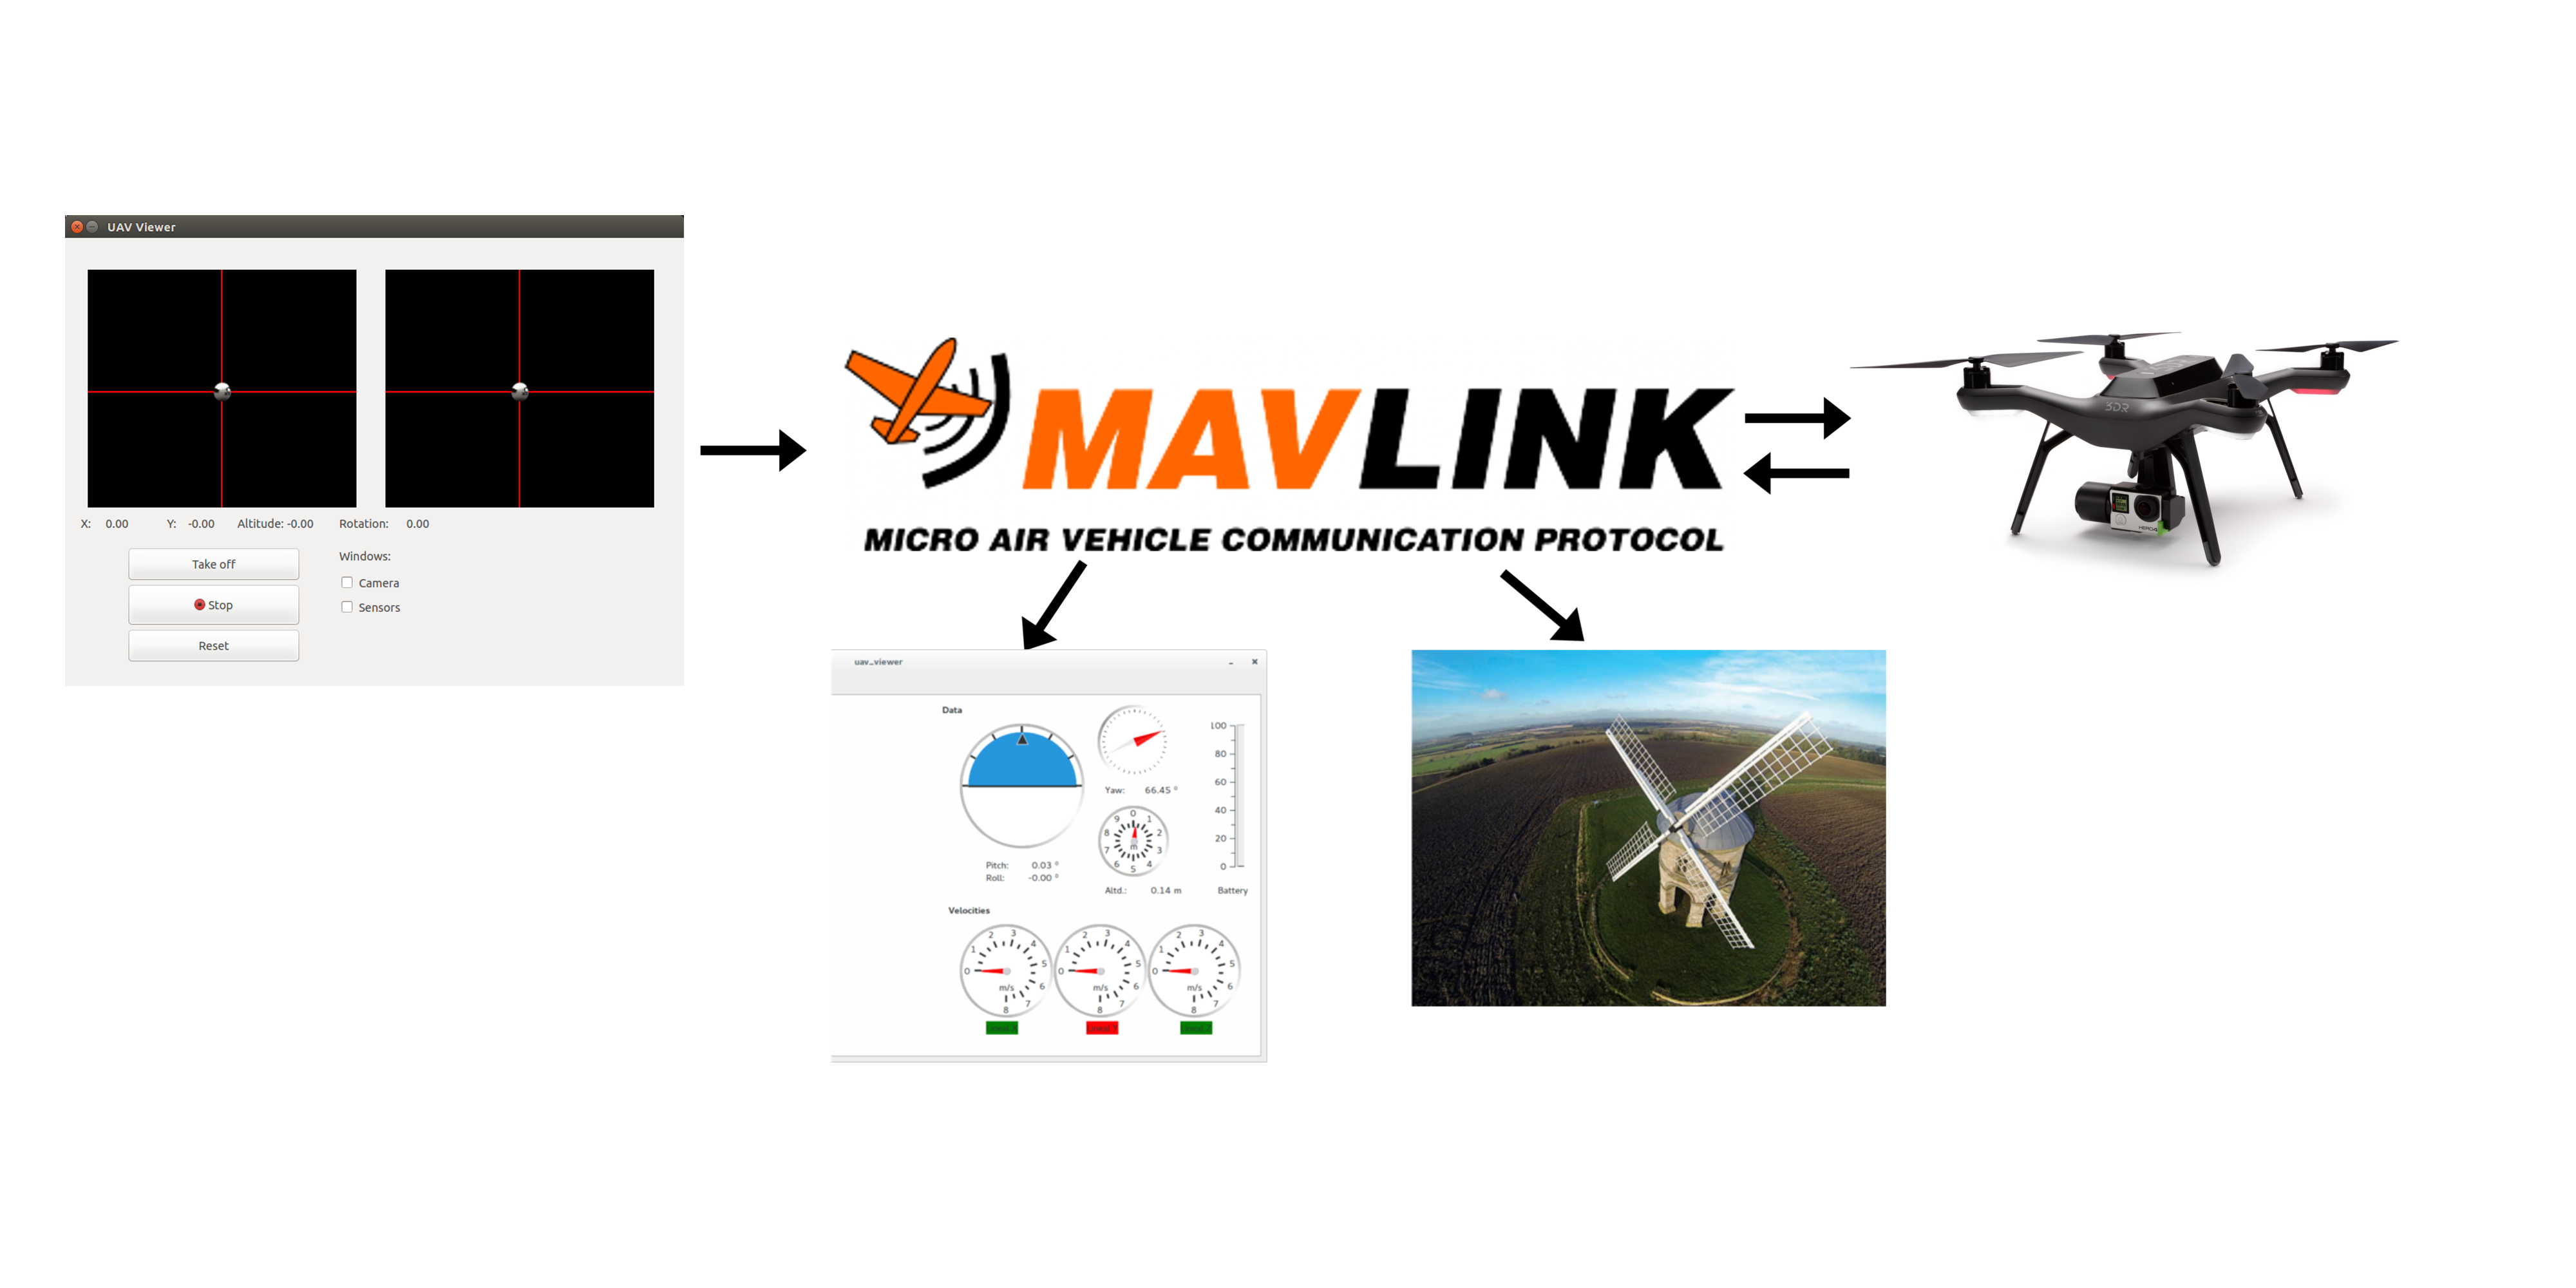
\includegraphics[scale=0.1]{imagenes/diagramaComunicacionServerDron1.png}
  \caption{Diagrama comunicación}
  \label{fig:diagramaComunicacionServerDron1}
\end{figure}


A continuación vamos a dividir en distintas fases el contenido de este driver y su ejecución:

\begin{itemize}
\item Diseño
\item Implementación
\item Operación
\end{itemize}

\section{Diseño}
\label{Diseno}
MAVLinkServer es un controlador basado en el software MAVProxy y desarrollado para actuar como un middleware de traducción. Ha sido diseñado como un controlador JdeRobot en lenguaje Python. Este módulo también es responsable de mantener la comunicación canales abiertos y actualizados, tanto en sentido ascendente como descendente. 

MAVLinkServer se basa en el analizador MAVProxy, la parte del programa que está a cargo de la administración de los mensajes de MAVLink. Establece la conexión con el piloto automático Pixhawk, Mantiene el canal de comunicación operativo, adquiere, interpreta mensajes, crea y envía mensajes nuevos con la información solicitada u ordenada por la aplicación.

El código desarrollado está principalmente a cargo de la gestión de las interfaces JdeRobot. Es capaz de manejar la información proporcionada por el lado de MAVProxy. Regula la creación y modificación de las clases donde la información se almacena temporalmente y abre canales de comunicación ICE para hacer que el módulo sea utilizable para aplicaciones JdeRobot.

Estos dos lados del módulo proporcionan un controlador fiable y multi-compatible con las características de ICE; MAVLinkServer puede conectarse con aplicaciones escritas en otros diferentes idiomas, como C ++, Python o Java, a través de las interfaces de JdeRobot. La figura \ref{fig:mavLinkJdeRobotNegra} representa un esquema de los bloques dentro de MAVLinkServer y sus conexiones a otras aplicaciones.

\begin{figure}[H]
  \centering
  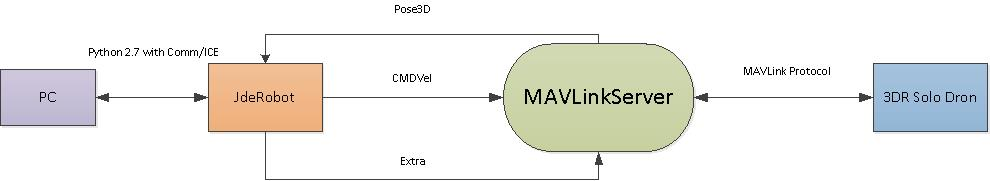
\includegraphics[scale=0.65]{imagenes/cajaNegra.jpg}
  \caption{Diagrama bloques MAVLink-JdeRobot}
  \label{fig:mavLinkJdeRobotNegra}
\end{figure}

MAVProxy es un sistema de comunicación grupal totalmente funcional  para drones. Es un sistema minimalista, portátil y extensible para cualquier UAV que soporte el protocolo MAVLink. Tiene una serie de características clave, que incluyen la capacidad de reenviar mensajes de UAV a través de la red a través de UDP o TCP a otros programas de estación terrestre en otros dispositivos.

\begin{itemize}
\item Es una aplicación de línea de comandos y consola. Hay complementos incluidos en MAVProxy para proporcionar una GUI básica.
\item Está escrito en Python.
\item Es de código abierto.
\item Es portátil; debería ejecutarse en cualquier sistema operativo POSIX con python, pyserial y función llamadas, lo que significa Linux, OS X, Windows y otros.
\item Admite módulos cargables, y tiene módulos para admitir consolas, mapas en movimiento, joysticks, seguidores de antena, etc.
\end{itemize}

Las interfaces JdeRobot utilizadas en este proyecto son Pose3D (proporciona la posición y medidas del vehículo), CMDVel (para enviar los comandos de velocidad) y Extra (para despegue y aterrizaje). Tenga en cuenta que Pose3D hace uso de cuaterniones en lugar de ángulos de Euler. Esto se hace para evitar singularidades angulares y superposiciones, y computacionalmente son más simples que otros formalismos de posicion como ángulos de Euler o una matriz de coseno de dirección.

\bigskip
\textbf{Pose3D:}
\begin{lstlisting}[frame=single]
  class Pose3DData
  {
		float x;
		float y;
		float z;
  	float h;
		float q0;
		float q1;
		float q2;
		float q3;
  };
\end{lstlisting}

\textbf{CMDVel:}
\begin{lstlisting}[frame=single]
	class CMDVelData
	{
		float linearX;
		float linearY;
		float linearZ;
		float angularX;
		float angularY;
		float angularZ;										
	};
\end{lstlisting}

\textbf{Extra:}
\begin{lstlisting}[frame=single]
	interface ArDroneExtra{
		void toggleCam();
		void land();
		void takeoff();
		void reset();
		void recordOnUsb(bool record);
		void ledAnimation(int type,float duration, float req);
		void flightAnimation(int type, float duration);
		void flatTrim();
	};
\end{lstlisting}

\section{Implementación}
\subsection{Pre-Configuración}
\label{Pre-Configuracion}
En este apartado nos vamos a centrar en explicar todo lo relacionado con los pasos a seguir para realizar una configuración, que nos puede ofrecer dependiendo de este tipo de configuración y todas las librerías que tenemos a nuestra disposición.

Para llevar a cabo esta configuración del servidor debemos tener en cuenta la existencia de una serie de ficheros, llamados módulos (en lenguajes como java, suelen conocerse con el nombre de librerías), que cada uno de ellos nos va a facilitar una utilidad diferente, que pueden ir desde conocer la batería, altura del dron o configurar una web-cam.

Estos módulos se pueden descargar desde el repositorio oficial de MAVLink o crear una librería propia e implementarla. En el siguiente código que se muestra se puede ver como esta implementa obtener la información de la batería a través del voltaje que desprende:
\footnote{\url{https://github.com/ArduPilot/MAVProxy}}.

\begin{lstlisting}[frame=single]
    def vcell_to_battery_percent(self, vcell):
        '''convert a cell voltage to an approximate
        percentage battery level for a LiPO'''
        if vcell > 4.1:
            # above 4.1 is 100% battery
            return 100.0
        elif vcell > 3.81:
            # 3.81 is 17% remaining, from flight logs
            return 17.0 + 83.0 * (vcell - 3.81) / (4.1 - 3.81)
        elif vcell > 3.2:
            # below 3.2 it degrades fast. It's dead at 3.2
            return 0.0 + 17.0 * (vcell - 3.20) / (3.81 - 3.20)
        # it's dead or disconnected
        return 0.0
\end{lstlisting}

El fichero de configuración que usa el servidor únicamente se limita a establecer los puertos mediante los cuales se va a realizar la comunicación de cara a un usuario. Esta comunicación la realiza mediante las interfaces ICE que permite la comunicación con el servidor, pudiendo así recibir datos de sensores y motores, y enviar las instrucciones de velocidad necesarias en cada momento.


\subsection{Script de arranque}
\label{Script de arranque}

El script de arranque se encargara de ejecutar todos los comandos previos y el servidor. El script se encuentra en MAVProxy/MAVProxyWinLAN.sh, deberemos averiguar la IP que levanta el dron, en nuestro caso, con el 3DR Solo, dicha IP la levanta el mando como hemos comentado en la introducción de este capitulo. Deberemos modificar el script con la IP del dron a la que nos hayamos conectado y ejecutarlo sin parámetros adicionales. El fichero README del repositorio contiene una descripción mas detallada de un ejemplo de ejecución.

Se necesita tener preinstalado tanto pyserial como una versión de pyvmavlink superior a la 1.1.50. Se realiza una descarga de todos los módulos, construye un directorio llamado MavProxy.egg en /home/USER/.local/python3.5/site-packages con el fin de tener almacenados todos los paquetes necesarios y con permisos suficientes. 

A través de estos paquetes generados es posible acceder a los comandos que nos proporciona MAVLink. A continuación se proporciona un listado de los posibles comandos opcionales que se pueden añadir al script de arranque y una breve explicación de cada uno de ellos se realizará en la sección \ref{operacion} bajo la tabla \ref{scriptArranqueComandos}.

\subsection{MAVLinkServer}

El primer paso es definir las interfaces correspondientes (explicadas en la sección 5.1). MAVLinkServer suministra todas las interfaces JdeRobot para el acceso de drones desde cualquier componente externo. Aquí está un ejemplo de la interfaz Pose3D.

\begin{lstlisting}[frame=single]
import jderobot, time, threading

lock = threading.Lock()

class Pose3DI(jderobot.Pose3D):

    def __init__(self,_x,_y,_z,_h,_q0,_q1,_q2,_q3):

        self.x = _x
        self.y = _y
        self.z = _z
        self.h = _h
        self.q0 = _q0
        self.q1 = _q1
        self.q2 = _q2
        self.q3 = _q3

        print ("Pose3D start")

    def setPose3DData(self, data, current=None):

        lock.acquire()

        self.x = data.x
        self.y = data.y
        self.z = data.z
        self.h = data.h
        self.q0 = data.q0
        self.q1 = data.q1
        self.q2 = data.q2
        self.q3 = data.q3

        lock.release()

        return 0

    def getPose3DData(self, current=None):

        time.sleep(0.05) # 20Hz (50ms) rate to tx Pose3D

        lock.acquire()

        data = jderobot.Pose3DData()
        data.x = self.x
        data.y = self.y
        data.z = self.z
        data.h = self.h
        data.q0 = self.q0
        data.q1 = self.q1
        data.q2 = self.q2
        data.q3 = self.q3

        lock.release()

        return data
\end{lstlisting}  

Esta clase hereda "jderobot.Pose3D" y se definen las funciones correspondientes. Eso
se puede notar el uso de "bloqueos" de programación para proteger los datos almacenados en la clase. Esto se debe a que MAVLinkServer actualiza constantemente la información provista por los sensores y también la publica constantemente a través de ICE. Esto podría causar condiciones de carrera. Con el uso de los bloqueos en las clases, la información no se podía leer mientras otra tarea estaba escribiendo en ella y viceversa, asegurando la administración correcta de la información en exclusión mutua.

MAVLinkServer lanza varios hilos para canales de comunicación ICE, uno para cada tipo de información. A pesar de que solo Pose3D, CMDVel y Extra deben ser realmente utilizados, el driver ofrece las interfaces restantes para compatibilidad y usos futuros.

Cada subproceso hace uso de su propia función donde se realiza la configuración de ICE.
Allí se realiza la publicación de ICE y es importante garantizar qué datos se envían, para que otras aplicaciones obtengan la información correctamente y garanticen la compatibilidad.
El mismo procedimiento se realiza para todas las interfaces.

\begin{figure}[H]
  \centering
  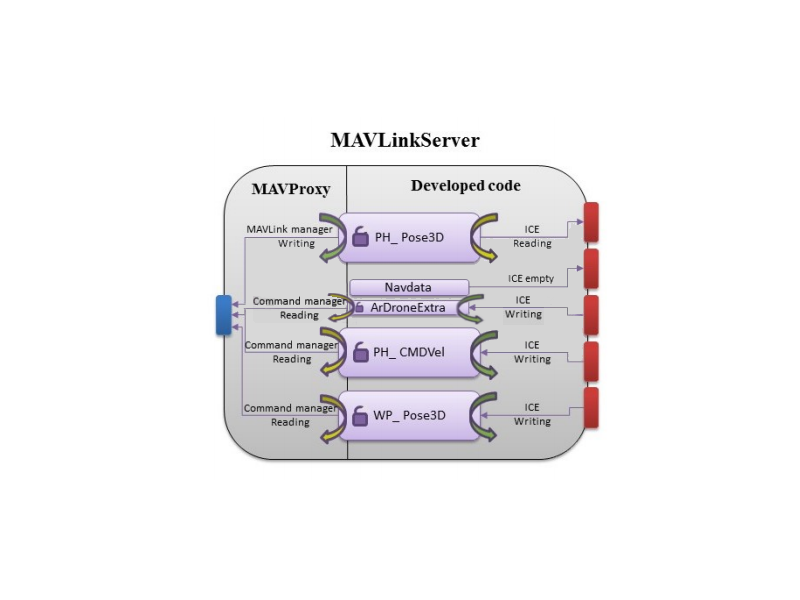
\includegraphics[scale=0.6]{imagenes/MavProxyPorDentro.png}
  \caption{Gestión de memoria}
  \label{fig:MavProxyInside}
\end{figure}

La interfaz CMDVel y Extra tiene la misma estructura que Pose3D, también con el uso de bloqueos.

\begin{lstlisting}[frame=single]

import jderobot, time, threading

lock = threading.Lock()

class CMDVelI(jderobot.CMDVel):

    def __init__(self,lx,ly,lz,ax,ay,az):

        self.linearX = lx
        self.linearY = ly
        self.linearZ = lz
        self.angularX = ax
        self.angularY = ay
        self.angularZ = az

        #print ("cmdvel start")

    #def __del__(self):

        #print ("cmdvel end")


    def setCMDVelData(self, data, current=None):

        lock.acquire()

        self.linearX = data.linearX
        self.linearY = data.linearY
        self.linearZ = data.linearZ
        self.angularX = data.angularX
        self.angularY = data.angularY
        self.angularZ = data.angularZ

        lock.release()

        return 0

    def getCMDVelData(self, current=None):

        time.sleep(0.05)  # 20Hz (50ms) rate to rx CMDVel

        lock.acquire()

        data = jderobot.CMDVelData()
        data.linearX = self.linearX
        data.linearY = self.linearY
        data.linearZ = self.linearZ
        data.angularX = self.angularX
        data.angularY = self.angularY
        data.angularZ = self.angularZ
        lock.release()

        return data
        
\end{lstlisting} 

\begin{lstlisting}[frame=single]
import jderobot, time, threading

lockLand = threading.Lock()
lockTakeOff = threading.Lock()

class ExtraI(jderobot.ArDroneExtra):

    def __init__(self):

        print ("Extra start")
        self.landDecision = False
        self.takeOffDecision = False

    def land(self,xxx):
        self.setLand(True)
        lockLand.acquire()
        landDecision = self.landDecision
        lockLand.release()

        return landDecision

    def takeoff(self,xxx):
        self.setTakeOff(True)
        lockTakeOff.acquire()
        takeOffDecision = self.takeOffDecision
        lockTakeOff.release()

        return takeOffDecision

    def setLand(self,decision):
        lockLand.acquire()
        self.landDecision = decision
        lockLand.release()

    def setTakeOff(self, decision):
        lockTakeOff.acquire()
        self.takeOffDecision = decision
        lockTakeOff.release()

    def setExtraData(self, data, current=None):

        lockLand.acquire()
        self.landDecision = data.landDecision
        lockLand.release()

        lockTakeOff.acquire()
        self.takeOffDecision = data.takeOffDecision
        lockTakeOff.release()

        return 0

\end{lstlisting}  
Por otro lado solo tiene una conexión con el puerto de comunicación con el dron (puerto serie). La gestión de estos 3 hilos de comunicación, respecto al único puerto serie que se mantiene por parte del dron, se basa en la gestión de prioridades. Extra es el más prioritario al ser el componente más restrictivo, este componente predomina sobre los otros 2 debido a la importancia de las ordenes que envía. Pose3D recibe la información del dron para actualizar la posición en un canal unicamente de lectura del puerto serie. Por otro lado conviven al mismo tiempo tanto CMDVel como Pose3D a la hora de realizar enviar comandos de velocidad y/o posición.

\begin{lstlisting}[frame=single]
	mpstate.status.thread = threading.Thread(target=main_loop, 
    						name='main_loop')
    mpstate.status.thread.daemon = True
    mpstate.status.thread.start()

    #Open an ICE TX communication and leave it open in a parallel threat

    PoseTheading = threading.Thread(target=openPose3DChannel, 
    				args=(PH_Pose3D,), name='Pose_Theading')
    PoseTheading.daemon = True
    PoseTheading.start()

    # Open an ICE RX communication and leave it open in a parallel threat

    CMDVelTheading = threading.Thread(target=openCMDVelChannel, 
    				args=(PH_CMDVel,), name='CMDVel_Theading')
    CMDVelTheading.daemon = True
    CMDVelTheading.start()

    # Open an ICE TX communication and leave it open in a parallel threat

    CMDVelTheading = threading.Thread(target=openExtraChannel, 
    				args=(PH_Extra,), name='Extra_Theading')
    CMDVelTheading.daemon = True
    CMDVelTheading.start()

    # Open an ICE channel empty

    CMDVelTheading = threading.Thread(target=openNavdataChannel, 
    					args=(), name='Navdata_Theading')
    CMDVelTheading.daemon = True
    CMDVelTheading.start()

    # Open an MAVLink TX communication and leave it open in a parallel 
    # threat
    #
    PoseTheading = threading.Thread(target=sendCMDVel2Vehicle, 
    				args=(PH_CMDVel,PH_Pose3D,), 
                    name='TxCMDVel_Theading')
    PoseTheading.daemon = True
    PoseTheading.start()


    # Open an ICE TX communication and leave it open in a parallel threat

    PoseTheading = threading.Thread(target=openPose3DChannelWP, 
    				args=(WP_Pose3D,), 
                    name='WayPoint_Theading')
    PoseTheading.daemon = True
    PoseTheading.start()

    # Open an MAVLink TX communication and leave it open in a parallel threat

    PoseTheading = threading.Thread(target=sendWayPoint2Vehicle,
    				args=(WP_Pose3D,), 
                    name='WayPoint2Vehicle_Theading')
    PoseTheading.daemon = True
    PoseTheading.start()

    # Open an MAVLink TX communication and leave it open in a parallel threat

    PoseTheading = threading.Thread(target=landDecision, 
    				args=(PH_Extra,), 
                    name='LandDecision2Vehicle_Theading')
    PoseTheading.daemon = True
    PoseTheading.start()
   
\end{lstlisting}

MAVproxy está constantemente manejando los mensajes MAVLink en un hilo paralelo en un bucle infinito. Este módulo lo aprovecha y refresca la información del sensor necesario. Como un controlador de alto nivel, este programa no interfiere con la fusión de datos realizado por Pixhawk y confía en su rendimiento, cuya fiabilidad ha sido ampliamente probado.

En el arranque del servidor se cargan los paquetes comentados en \ref{scriptArranqueComandos} y a partir de los cuales se podrán proporcionar funcionalidades, un ejemplo es el modo consola, el cual nos permite controlar al dron a partir de comandos definidos en la lista \ref{comandos}, que se comentará más en detalle en la sección \ref{operacion}.

\begin{figure}[H]
  \centering
  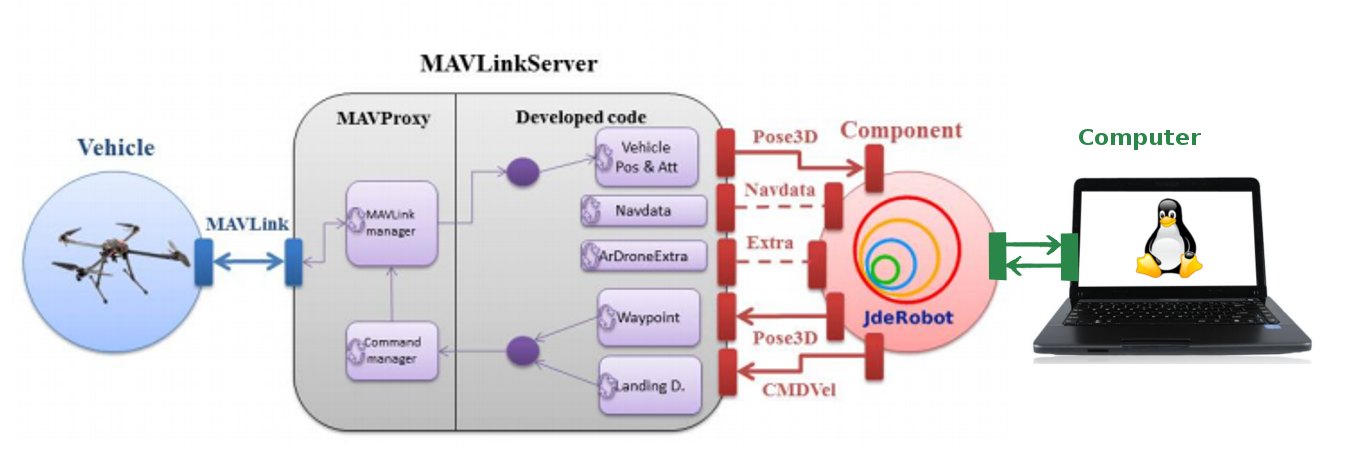
\includegraphics[scale=0.35]{imagenes/cajaTrasparente.png}
  \caption{Diagrama bloques MAVLink-JdeRobot con detalle}
  \label{fig:mavLinkJdeRobotTrasparente}
\end{figure}


Para llevar a cabo esta carga el primer paquete que se carga es "Link", este paquete se encarga de la conexión entre el servidor y el dron. Es necesario conocer la dirección IP que levanta este dron, que ya habremos configurado en el paso \ref{Script de arranque}. Tras lograr la conexión se establece un periodo de "checkeo" necesario para no perder la conexión con el dron en caso de llegar a una distancia límite o un fallo de conexión, en cuyo caso se procede a detenerse el dron. Esto se debe a periódicamente se debe realizar una comunicación entre el dron y el servidor, aunque no se llegue a mandar ningún comando, ya sea de velocidad o algún tipo de acción, el servidor por su parte comunicara que aun esta conectado. Después de un tiempo sin conexión, aproximadamente unos 10-15 segundos, el dron procederá a realizar un despegue. 



\begin{lstlisting}[frame=single]
def periodic_tasks():
    '''run periodic checks'''
    if mpstate.status.setup_mode:
        return

    if (mpstate.settings.compdebug & 2) != 0:
        return

    if mpstate.settings.heartbeat != 0:
        heartbeat_period.frequency = mpstate.settings.heartbeat

    if heartbeat_period.trigger() and mpstate.settings.heartbeat != 0:
        mpstate.status.counters['MasterOut'] += 1
        for master in mpstate.mav_master:
            send_heartbeat(master)

    if heartbeat_check_period.trigger():
        check_link_status()

    set_stream_rates()

    for (m,pm) in mpstate.modules:
        if hasattr(m, 'idle_task'):
            try:
                m.idle_task()
            except Exception as msg:
                if mpstate.settings.moddebug == 1:
                    print(msg)
                elif mpstate.settings.moddebug > 1:
                    exc_type, exc_value, exc_traceback = sys.exc_info()
                    traceback.print_exception(exc_type, exc_value, 
                    		exc_traceback,limit=2, file=sys.stdout)

        # also see if the module should be unloaded:
        if m.needs_unloading:
            unload_module(m.name)
\end{lstlisting}
            
Al acabar toda la carga de los módulos establecemos la conexión con los puertos necesarios con JdeRobot para poder pilotar el dron. Los módulos que usamos son Pose3D, CMDVel y Extra. Para cada uno de ellos vamos a necesitar crear 2 threads, uno para establecer la conexión con un sistema externo, en nuestro caso será el visor UavViewer, y otro para recibir los comandos que nos deseen enviar por el canal. Cada módulo lo necesitaremos por los siguientes motivos:

\begin{lstlisting}[frame=single]

def load_module(modname, quiet=False):
    '''load a module'''
    modpaths = ['MAVProxy.modules.mavproxy_%s' % modname, modname]
    for (m,pm) in mpstate.modules:
        if m.name == modname:
            if not quiet:
                print("module %s already loaded" % modname)
            return False
    for modpath in modpaths:
        try:
            m = import_package(modpath)
            imp.reload(m)
            module = m.init(mpstate)
            if isinstance(module, mp_module.MPModule):
                mpstate.modules.append((module, m))
                if not quiet:
                    print("Loaded module %s" % (modname,))
                return True
            else:
                ex = "%s.init did not return a MPModule instance" % modname
                break
        except ImportError as msg:
            ex = msg
            if mpstate.settings.moddebug > 1:
                import traceback
                print(traceback.format_exc())
    print("Failed to load module: %s. Use 'set moddebug 3' in the MAVProxy console to enable traceback" % ex)
    return False
\end{lstlisting}

\begin{itemize}
\item CMDVel: Este módulo nos dará lo necesario para poder mover el dron en los ejes x,y,z y sobre el yaw. La velocidad máxima que se le puede dar al dron a través del interfaz UavViewer en cada dirección viene dado en una escala de 0 a 1.  
\begin{lstlisting}[frame=single]
def sendCMDVel2Vehicle(CMDVel,Pose3D):
    absolute = 0
    relative = 1

    while True:

        CMDVel2send = CMDVel.getCMDVelData()
        Pose3D2send = Pose3D.getPose3DData()
        #print(Pose3D2send)
        NEDvel = body2NED(CMDVel2send, Pose3D2send) # [x,y,z]
        linearXstring = str(NEDvel[0])
        linearYstring = str(NEDvel[1])
        linearZstring = str(NEDvel[2])

        #CMDVel.angularZ -1 y 1

        angular = CMDVel.angularZ

        if angular >= 0:
            direction = str(1)
        else:
            angular = -angular
            direction = str(-1)

        angularZstring = str(angular*30)

        movement = str(relative)

        velocitystring = 'velocity '+ linearXstring + ' ' + 
        				  linearYstring + ' ' + 
                          linearZstring
        angularString = 'setyaw ' + angularZstring + ' ' + 
        				  direction + ' ' + movement

        process_stdin(velocitystring) 
        process_stdin(angularString)
\end{lstlisting}
\item Extra: Este módulo nos dará la facilidad de despegar y de aterrizar. Debido al protocolo MAVLink, el sistema de despegue se compone en 3 fases, que con nuestro UavViewer se agrupan todas ellas. Durante la fase de despegue el dron no admite ningún comando a excepción del comando "land" para aterrizar, o en caso del despegue, para detener el despegue.  Este despegue dura aproximadamente unos 10 segundos hasta que se estabiliza en el aire por motivos de seguridad. \begin{enumerate}
						\item El arranque de las hélices. 
                        \item Despegue del dron.
                        \item Habilitar comandos de velocidad.
						\end{enumerate}
\item Pose3d: Este módulo nos indicara la posición del dron en todo momento, así como su orientación y altitud. Esta conexión nos va a servir tanto a la hora de aterrizar y despegar usando el otro módulo comentado Extra, para saber si puede aterrizar en un determinado momento o debe disminuir su altura antes de parar los motores.

\end{itemize}

\section{Operación}
\label{operacion}
En esta sección se va a explicar la posible configuración que permite el MAVLinkServer. Esta configuración se puede realizar en 2 niveles, a nivel del script de arranque o a partir de comandos una vez que el servidor este arrancado.

La configuración que se puede modificar a nivel de script esta relacionada con el tipo de conexión que se quiere mantener con el dron. Esta conexión tiene valores por defecto pero se puede modificar si asi se desea. Los comandos que se muestran en la tabla \ref{scriptArranqueComandos} son un ejemplo de la versatilidad que tiene el servidor:

\begin{multicols}{2}
\begin{itemize}
\label{scriptArranqueComandos}
\item master: Puerto maestro MAVLink y baudrate opcional. Por defecto=[].
\item udp: Arranca el servidor udp. Por defecto se elige TCP.
\item tcp: Arranca el servidor tcp. Por defecto se elige TCP.
\item out: Puerto de salida MAVLink. Por defecto=[].
\item baudrate: Por defecto=57600.
\item sitl(Software in the loop): Puerto de salida, esta opción únicamente es necesaria en caso de no tener disponible un dron.
\item streamratedest: MAVLink stream rate. Por defecto=4.
\item source-system: Código fuente MAVLink. Por defecto=255.
\item source-component: Componente origen MAVLink. Por defecto=0.
\item target-system: Sistema destino MAVLink. Por defecto=0.
\item target-component: Componente destino MAVLink. Por defecto=0.
\item logfile: Fichero de logs. Por defect=mav.tlog
\item append-log (También aceptado "-a"): Añadir al fichero de log ya existente. Por defecto=False.
\item continue (También aceptado con "-c"): Continua el log. Por defecto=False.
\item quadcopter: Usar acciones de control para cuadricopteros. Por defecto=False.
\item setup: Arrancar en modo setup. Por defecto=False.
\item nodtr: Deshabilitar DTR(Data Terminal Ready). Por defecto=False.
\item show-errors: Mostrar errores MAVLink. Por defecto=False.
\item speech: Usar texto para hablar. Por defecto=False.
\item aircraft: Establecer nombre para el dron (Visual en mensajes). Por defecto=None.
\item cmd: Comandos a ejecutar tras el arranque. Por defecto=None.
\item console: Usar consola GUI para introducir comandos. 
\item map: Carga un mapa de la zona.
\item load-module: Carga un modulo especifico, puede ser utilizado tantas veces como sea necesario separando con ","). Por defecto=[].
\item mav09: Usa protocolo MAVLink 0.9. Por defecto=False.
\item auto-protocol: Auto detecta versión de protocolo MAVLink. Por defecto=False.
\item nowait: No realiza comunicación continua con el dron (HearthBeat). Por defecto=False.
\item dialect: Dialecto MAVLink. Por defecto=ardupilotmega.
\item rtscts: Habilita control de comunicación vía RTS/CTS.
\item moddebug  type=int, help="module debug level default=0
\item mission: Nombre de la misión. Por defecto=None.
\item daemon: Arranca en modo daemon, no muestra shell interactiva.
\item profile: Arranca el Yappi python profiler.
\item state-basedir: Directorio base para logs. Por defecto=None.
\item version: Muestra información sobre la versión.
\item default-modules: Módulos por defecto al iniciar. Por defecto=log, wp, rally, fence, param, relay, tuneopt, arm, mode, calibration, rc, auxopt, misc, cmdlong, battery, terrain, output.
\end{itemize}
\end{multicols}

Los comandos que se muestran en la tabla \ref{comandos}, solo se pueden ejecutar si en el paso anterior se ha introducido el comando "--console", de cualquier otra manera, no se muestra la consola mediante la cual se pueden introducir comandos. Estos comandos tienen una labor de modificar la experiencia de vuelo del dron o muestra los valores que nos pueden proporcionar sus sensores:

\begin{itemize}
\label{comandos}
\item reboot: Reinicia el dron.
\item arm: Habilita los medidores propios del dron. Ejemplo de ejecución: check (all|baro|compass|gps|ins|params|rc|voltage|battery),uncheck (all|baro|compass|gps|ins|params|rc|voltage|battery),list,throttle,safetyon,safetyoff (arm throttle arranca hélices del dron)
\item disarm: Detiene los motores del dron.
\item takeoff: Despegue del dron.
\item land: Aterrizaje del dron.
\item mode: Cambia el modo de vuelo.
\item velocity: Establece una velocidad en los ejes x,y,z. Ejemplo de ejecución: velocity 1 0 0
\item parachute: Habilita un aterrizaje del dron si pierde conexión o la batería es baja. Ejemplo de ejecución: parachute [enable|disable|release]
\item bat: Muestra batería del dron.
\item alt: Muestra altitud del dron.
\end{itemize}
